\documentclass[a4paper,12pt]{article}
\usepackage[utf8]{inputenc}
\usepackage{url}
\usepackage{hyperref}
\usepackage[english,brazil]{babel}
\usepackage{comment}
\usepackage{bookmark}
\usepackage{graphicx}


\title{Estratégias de Sintetização de Voz utilizando Deep Learning para Leitura Humanizada de Textos}
\author{
  Aluno: Thomaz Diniz\\
  \texttt{thomaz.morais@ccc.ufcg.edu.br}
  \and
  Orientador: Herman Martins\\
  \texttt{hmg@computacao.ufcg.edu.br}
}
\date{}


\begin{document}	
	\maketitle
	\selectlanguage{english}
	\begin{abstract}
		Text-to-speech (TTS) is an extremely important tool in the pursuit of accessibility. It benefits not only people with visual impairments but also those with difficulties in reading comprehension. Recent advancements in deep learning enable the synthesis of voice with quality very close to recordings made by humans. In this study, we aim to replicate state-of-the-art techniques used to synthesize voices within the context of Brazilian Portuguese.
		
		Keywords: Deep learning, Acessibility
	\end{abstract}


	\selectlanguage{brazil}
	\begin{abstract}
		A síntese de fala a partir de texto é uma ferramenta crucial para promover a acessibilidade. Não apenas beneficia pessoas com deficiência visual \cite{WAI_2024_guidlines_for_accessibility}, mas também aquelas com dificuldades na compreensão de textos \cite{wood2017readingaccessibility}. Avanços recentes no campo do deep learning têm possibilitado a geração de voz sintética com qualidade comparável à de gravações humanas \cite{tan2022naturalspeech}. Neste estudo visamos replicar técnicas de  síntese de voz para o contexto do português brasileiro.
		
		Palavras-chave: Deep learning, Acessibilidade
	\end{abstract}


	\selectlanguage{english}
	
	\section{Introdução}
	
		Avanços recentes na área de deep learning têm possibilitado o desenvolvimento de sistemas de síntese de voz humana de maneira cada vez mais precisa e natural. Tan et. al. por exemplo, produziram o NaturalSpeech, um modelo capaz de replicar a voz humana com uma qualidade idêntica a de gravações humanas \cite{tan2022naturalspeech}). Essa tecnologia oferece uma possibilidade de melhoria na acessibilidade digital. Recursos de acessibilidade de sintetização de voz a partir de textos (do inglês text-to-speech ou simplesmente TTS) são utilizadas a bastante tempo, mas ainda existe uma lacuna no impacto que ferramentas que se aproximam mais a dicção e a voz humana podem trazer na melhoria da qualidade de vida para pessoas com deficiência visual e dificuldade de compreensão de textos. Neste estudo pretendemos replicar técnicas de TTS  no português.

		\subsection{Objetivo}
		Este artigo propõe explorar síntese de voz humanizada utilizando técnicas de deep learning. Buscamos desenvolver sistemas TTS para tentar reproduzir a entonação, o ritmo e outras características da fala humana para o português brasileiro. Em um primeiro momento trataremos as tecnologias como caixa preta para entender os desafios iniciais dessas tecnicas.

		\subsection{Questões de Pesquisa}
		\begin{itemize}
			\item Quais são as técnicas mais eficazes de deep learning para desenvolver TTS em português mais humanizada (entonação, ritmo e outras características)?
			\item Como validar e avaliar o quão humanizada está a leitura do texto obtida pelo TTS?
		\end{itemize}
	\section{Revisão da Literatura}
		\subsection{Artigos Selecionados}
			\subsubsection{Artigo 1: TACOTRON: TOWARDS END-TO-END SPEECH SYNTHESIS}
			
			Contexto e contribuições:
						
			O contexto do artigo é de text-to-speech (tts) ou síntese de voz a partir de texto. Nele é difinida uma arquitetura onde o modelo recebe caracteres como input e retorna um espectograma. A partir deste espectograma é utilizada uma outra técnica chamda de WaveNet \cite{oord2016wavenet} para transformar o espectograma em audio utilizando uma reconstrução Griffin-Lim.
			
			Como a solução proposta pelo artigo foi avaliada?
			
			A solução foi avaliada através de uma survey de falantes nativos com Mean Opinion Score (MOS) comparando com outros modelos de TTS: O modelo Parametric \cite{zen2016parametric} e o modelo Concatenativa \cite{goncalvo2016concatenative}.
			
			Pontos fortes do artigo:
			\begin{itemize}
				\item Os modelos são bem claros, e o processo é bem explicado.
			\end{itemize}
			Pontos que o artigo poderia melhorar:
			\begin{itemize}
				\item Artigo não acompanha código.
				\item Artigo não acompanha modelo para facilitar a validação.
			\end{itemize}
			
			
			\subsubsection{Artigo 2: Conversão Texto-Fala para o Português Brasileiro Utilizando Tacotron 2 com Vocoder Griffin-Lim}
			
			Contexto e contribuições:
			
			Neste paper há uma aplicação do tacotron, mas dessa vez com foco no português. O artigo consegue aplicar o português, contudo o resultado é bem aquem do esperado com diversas vozes extremamente robóticas. \cite{rosa2021ttsptbr}

			Como a solução proposta pelo artigo foi avaliada?
			
			Os autores decidiram por fazer uma avaliação de quantidade de erros de pronúncia e palavras puladas. No artigo não há uma definição do que são palavras que foram puladas mas assumo que sejam palavras cujo modelo não foi capaz de pronunciar e simplesmente ignorou.
			
			Pontos fortes do artigo:
			\begin{itemize}
				\item O paper acompanha de um github com códigos, ou seja pode ser validado e replicado com certa facilidade.
			\end{itemize}
			Pontos que o artigo poderia melhorar:
			\begin{itemize}
				\item A validação parece ser uma estratégia boa para quando não se tem muitos recursos, mas ela é extremamente limitada a um modelo que espera-se que cometa erros muito fortes.
				\item Resultados das vozes geradas não são muito bons.
			\end{itemize}
			
			\subsubsection{Artigo 3: NaturalSpeech: End-to-End Text-to-Speech Synthesis with Human-Level Quality}
			
			Contexto e contribuições:
						
			O contexto também é de TTS, além de trazer a proposta de uma técnica de sintetização de voz, ele também se propõe a trazer uma maneira de definir e julgar o quão próximo o sintetizador de voz está do nível de qualidade de voz humana. E no artigo é dito que eles conseguem algo muito próximo da qualidade humana definindo um sintetizador de qualidade humana como: Um sintetizador que gera vozes em que não há diferença estatística entre uma gravação humana e a síntese de voz pela primeira vez em uma mean opinion score.
			
			Como a solução proposta pelo artigo foi avaliada?
			
			A solução foi avaliada através de uma survey de falantes nativos com escala MOS(mean opinion score) comparando com outros modelos de TTS: O modelo Parametric \cite{zen2016parametric} e o modelo Concatenativa \cite{goncalvo2016concatenative}. Este artigo foi escolhido não somente por ser estado da arte, como também por ter bastante fundamentação matemática e formalismo.
			
			Atividade 1 de FPCC3: A formalização a seguir explica um autoencoder variacional. O objetivo de um autoencoder variacional é codificar um input automaticamente em uma representação comprimida que pode depois ser decodificado para que o input possa ser reconstruído a partir do que foi codificado. Isso pode ser usado para explicar o processo de reconstrução de voz a partir de um treinamento utilizando este autoencoder. Em um primeiro momento é feita a codificação em algo que é chamado de vetor latente Z. Em um momento do artigo é feita a formalização matemática do autoencoder para explicar seu funcionamento.

			$X$: Voz original
			
			$Y$: Sequência de texto
			
			$q(z \mid x)$: Encoder que parametriza a distribuição dos dados X para a a variável latente Z.
			
			$p(x \mid z)$: Decoder que reconstrói o input que foi passado que no caso é o audio passado.
				
			$p(z \mid y)$: Um segundo encoder que codifica uma sequência de texto Y em fonemas. E será passado ao Decoder posteriormente
			
			$S: p(z \mid y) \rightarrow  p(x \mid z)$: Voz Sintetizada a partir do processo de decodificação onde em um primeiro momento se obtém o latente Z a partir do texto, para depois ser feita a decodificação do spectograma que é utilizado em um segundo momento para formar a voz em si.
			
\iffalse
			\begin{figure}[bp!]
				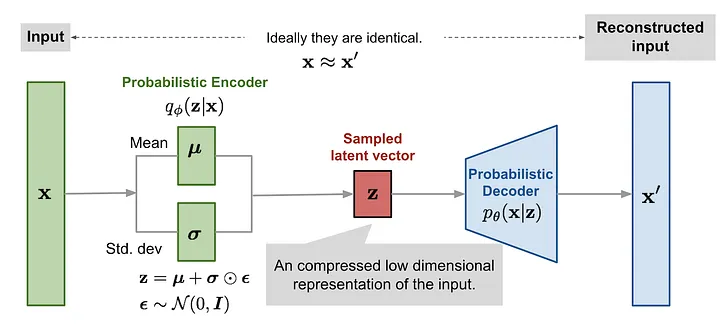
\includegraphics[width=\linewidth]{./imgs/encoder.png}
				\caption{Autoencoder}
				\label{fig:autoencoder}
			\end{figure}
			
			Figure \ref{fig:autoencoder} autoencoder.
				
\fi

			Pontos fortes do artigo:
			
			\begin{itemize}
				\item Acompanha código o que facilita na replicação.
			\end{itemize}
			Pontos que o artigo poderia melhorar:
			\begin{itemize}
				\item Muitos termos específicos da área, o que faz com que o artigo seja um pouco inacessível para alguém que está começando os estudos.
			\end{itemize}
			
	\section{Metodologia}
		\subsection{Tipo de Pesquisa}
		O tipo de pesquisa adotado que seguiremos serão os de experimentação e comparação. Onde em um primeiro momento testaremos múltiplas técnicas de síntese de voz, tentando entender os desafios para aplicá-las no contexto do português brasileiro e em um segundo momento realizaremos a comparação dos resultados.
		
		\subsection{Estudos Selecionados}
		Alguns dos estudos selecionados estão contidos na seção de revisão sistemática da literatura. Atualmente o Estado da arte é o NaturalSpeech, realizaremos experimentações com os modelos de deep learning do tacotron e de outros estudos também.
		
		\subsection{Extração dos dados}
		Para popular os nossa base de dados de vozes, utilizaremos o Fala Brasil \cite{falabrasil}, mas estamos em busca de outros bancos de vozes disponíveis gratuitamente online para este momento preliminar da pesquisa.

		\subsection{Validação}
		Parte dos nossos estudos iniciais vão ser para entender como validar as nossas experimentações. Alguns dos estudos que já mapeamos utilizam MOS(mean opinion score ou Pontuação média de opinião no português), que são parâmetros subjetivos feitos através de pesquisas com falantes nativos da linguagem. Para fazer a experimentação em si, utilizaremos código aberto das técnicas discutidas no artigo como caixa preta e manipularemos parâmetros de entrada para fazer comparações entre as técnicas e seus resultados. Estudaremos também possibilidades de algoritmos de comparação entre a voz sintetizada e um baseline de voz humana gravada.
	
	\bibliographystyle{ACM-Reference-Format}
	\bibliography{ref}

\end{document}